\documentclass[9pt,twocolumn,twoside,]{pnas-new}

% Use the lineno option to display guide line numbers if required.
% Note that the use of elements such as single-column equations
% may affect the guide line number alignment.


\usepackage[T1]{fontenc}
\usepackage[utf8]{inputenc}

% tightlist command for lists without linebreak
\providecommand{\tightlist}{%
  \setlength{\itemsep}{0pt}\setlength{\parskip}{0pt}}


% Pandoc citation processing
%From Pandoc 3.1.8
% definitions for citeproc citations
\NewDocumentCommand\citeproctext{}{}
\NewDocumentCommand\citeproc{mm}{%
  \begingroup\def\citeproctext{#2}\cite{#1}\endgroup}
\makeatletter
 % allow citations to break across lines
 \let\@cite@ofmt\@firstofone
 % avoid brackets around text for \cite:
 \def\@biblabel#1{}
 \def\@cite#1#2{{#1\if@tempswa , #2\fi}}
\makeatother
\newlength{\cslhangindent}
\setlength{\cslhangindent}{1.5em}
\newlength{\csllabelwidth}
\setlength{\csllabelwidth}{3em}
\newenvironment{CSLReferences}[2] % #1 hanging-indent, #2 entry-spacing
 {\begin{list}{}{%
  \setlength{\itemindent}{0pt}
  \setlength{\leftmargin}{0pt}
  \setlength{\parsep}{0pt}
  % turn on hanging indent if param 1 is 1
  \ifodd #1
   \setlength{\leftmargin}{\cslhangindent}
   \setlength{\itemindent}{-1\cslhangindent}
  \fi
  % set entry spacing
  \setlength{\itemsep}{#2\baselineskip}}}
 {\end{list}}
\usepackage{calc}
\newcommand{\CSLBlock}[1]{#1\hfill\break}
\newcommand{\CSLLeftMargin}[1]{\parbox[t]{\csllabelwidth}{#1}}
\newcommand{\CSLRightInline}[1]{\parbox[t]{\linewidth - \csllabelwidth}{#1}\break}
\newcommand{\CSLIndent}[1]{\hspace{\cslhangindent}#1}


\templatetype{pnasresearcharticle}  % Choose template

\title{Dynamique des communautés}

\author[a]{Kyara Boisvert}
\author[a]{Zoé Chol}
\author[a]{William Simard}

  \affil[a]{Université de Sherbrooke, Département d'écologie, 2500
Boulevard de l'Université, Sherbrooke, Québec, J1N 3C6}


% Please give the surname of the lead author for the running footer
\leadauthor{}

% Please add here a significance statement to explain the relevance of your work
\significancestatement{}


\authorcontributions{}



\correspondingauthor{\textsuperscript{} }

% Keywords are not mandatory, but authors are strongly encouraged to provide them. If provided, please include two to five keywords, separated by the pipe symbol, e.g:
 \keywords{  abondance |  taxonomie |  communautés |  séries
temporelles  } 

\begin{abstract}
La Terre sert d'habitat pour plusieurs espèces et chacune d'entre elles
ont une importance. Les écosystèmes retrouvés sur notre planète
permettent de créer un équilibre et notamment d'assurer la survie des
êtres humains. Cependant, les désirs humains sont parfois plus grands
que nécessaire et entre en conflit, causant la dégradation rapide des
écosystèmes, et d'important déclins dans les différentes populations,
allant même jusqu'à l'extinction de certaines espèces. De cette façon,
étudier l'état de la biodiversité est nécessaire afin déterminer les
solutions possibles et sensibiliser afin de conserver et préserver les
écosystèmes.
\end{abstract}

\dates{This manuscript was compiled on \today}
\doi{\url{www.pnas.org/cgi/doi/10.1073/pnas.XXXXXXXXXX}}

\begin{document}

% Optional adjustment to line up main text (after abstract) of first page with line numbers, when using both lineno and twocolumn options.
% You should only change this length when you've finalised the article contents.
\verticaladjustment{-2pt}



\maketitle
\thispagestyle{firststyle}
\ifthenelse{\boolean{shortarticle}}{\ifthenelse{\boolean{singlecolumn}}{\abscontentformatted}{\abscontent}}{}

% If your first paragraph (i.e. with the \dropcap) contains a list environment (quote, quotation, theorem, definition, enumerate, itemize...), the line after the list may have some extra indentation. If this is the case, add \parshape=0 to the end of the list environment.

\acknow{}

À travers le temps, les écosystèmes se sont formés grâce à une grande
diversité d'espèces animales et végétales. Cette richesse spécifique
retrouvée sur Terre, est intrinsèquement et de manière pragmatique
essentielle à la survie des êtres humains (1). Malgré la reconnaissance
de ces faits et des efforts de conservations constant au maintien de la
biodiversité, elle continue de décliner à un rythme alarmant (1, 2).
Plusieurs populations largement répandues ainsi que des espèces menacées
s'affaiblissent (3). Combiné avec l'exploitation humaine des écosystèmes
terrestres et des écosystèmes marins, ces facteurs résultent en un
biotope terrestre utilisé bien au-delà de sa durabilité (1). À la suite
d'analyses statistiques et d'observations d'une banque de données de
séries temporelles comportant des échantillonnages entre les années 1950
et 2020, incluant une variété de taxon végétal et animal, trois
questions de recherche ont émergées. La première : Observe-t-on un
déclin de la biodiversité à travers les années ? La deuxième : Quel
taxon est le plus et le moins observé à travers les années ? Puis la
dernière : Quel taxon a le plus décliné depuis les années 1970 ? Pour
répondre à ces questions, d'autres analyses statistiques ont été menée
évaluant l'abondance des différentes espèces retrouvées à travers les
années. La répartition de l'abondance des espèces permet d'obtenir des
preuves sur le niveau de rareté d'une espèce particulière relativement à
d'autres espèces (4).

\section{Méthodes}\label{muxe9thodes}

Afin de réaliser les analyses statistiques, la banque de données «
séries\_temporelles » fournie par Biodiversité Québec, a été utilisée.
Cette banque de données contient des données d'observations récoltées de
1950 à 2020 et leurs données taxonomiques associées. Pour débuter, les
données d'observations et les données relatives à la taxonomie ont été
importées dans le logiciel R dans des objets distincts. Ces données
sont, par la suite, passés par un processus de nettoyage et de
validation de manière à avoir une base de données utilisable pour les
analyses. Sur ces bases de données, trois dataframes ont été créé pour
séparer et regrouper les informations liées, ils regroupent
respectivement les informations de taxonomie, de référence et
d'observations. Après avoir créé trois tables vides correspondantes dans
un serveur SQL, ces dataframes ont été utilisés pour injecter les
données dans la base de données SQL et remplir les tables. C'est ainsi
cette base de données permet d'effectuer les analyses statistiques et la
visualisation des données. De ce fait, les trois figures suivantes ont
été créées. La Figure \ref{fig:esp.annee} a été conçue à l'aide de la
fonction ``plot''. Le type de lignes, l'épaisseur de la ligne ainsi que
la couleur de celles-ci ont été défini selon les caractéristiques
désirées. Ce graphique représente la richesse spécifique par année selon
le nombre d'espèces observées. La Figure \ref{fig:obs.classe}, est un
graphique à barres conçu à l'aide de la fonction ``bar plot'', qui
représente les différentes classes taxonomiques ainsi que le nombre
d'observation sur une échelle logarithmique. Des caractéristiques
spécifiques telles que la couleur des bandes et leurs bordures ont été
attribués. Enfin, la Figure \ref{fig:declin} est également un graphique
à barres représentant les variations, en pourcentage, des espèces
observées selon les différentes classes à partir des années 1970. Les
bandes rouges représentent les diminutions en abondance des espèces et
les bandes vertes sont les augmentations depuis 1970 selon chaque classe
taxonomique observée.

\section{Résultats}\label{ruxe9sultats}

Les analyses ont démontré une augmentation dans la richesse spécifique
entre les années 1950 et \textasciitilde{} 1993 (Figure
\ref{fig:esp.annee}). De plus, une forte augmentation du nombre
d'espèces observées est notable dans les années 1970. Cependant, un
déclin dans l'abondance des espèces à partir de l'année 1995 est
également visible, suivi de quelques hausses, mais d'une tendance
générale au déclin s'aggravant d'années en années.

\begin{figure}
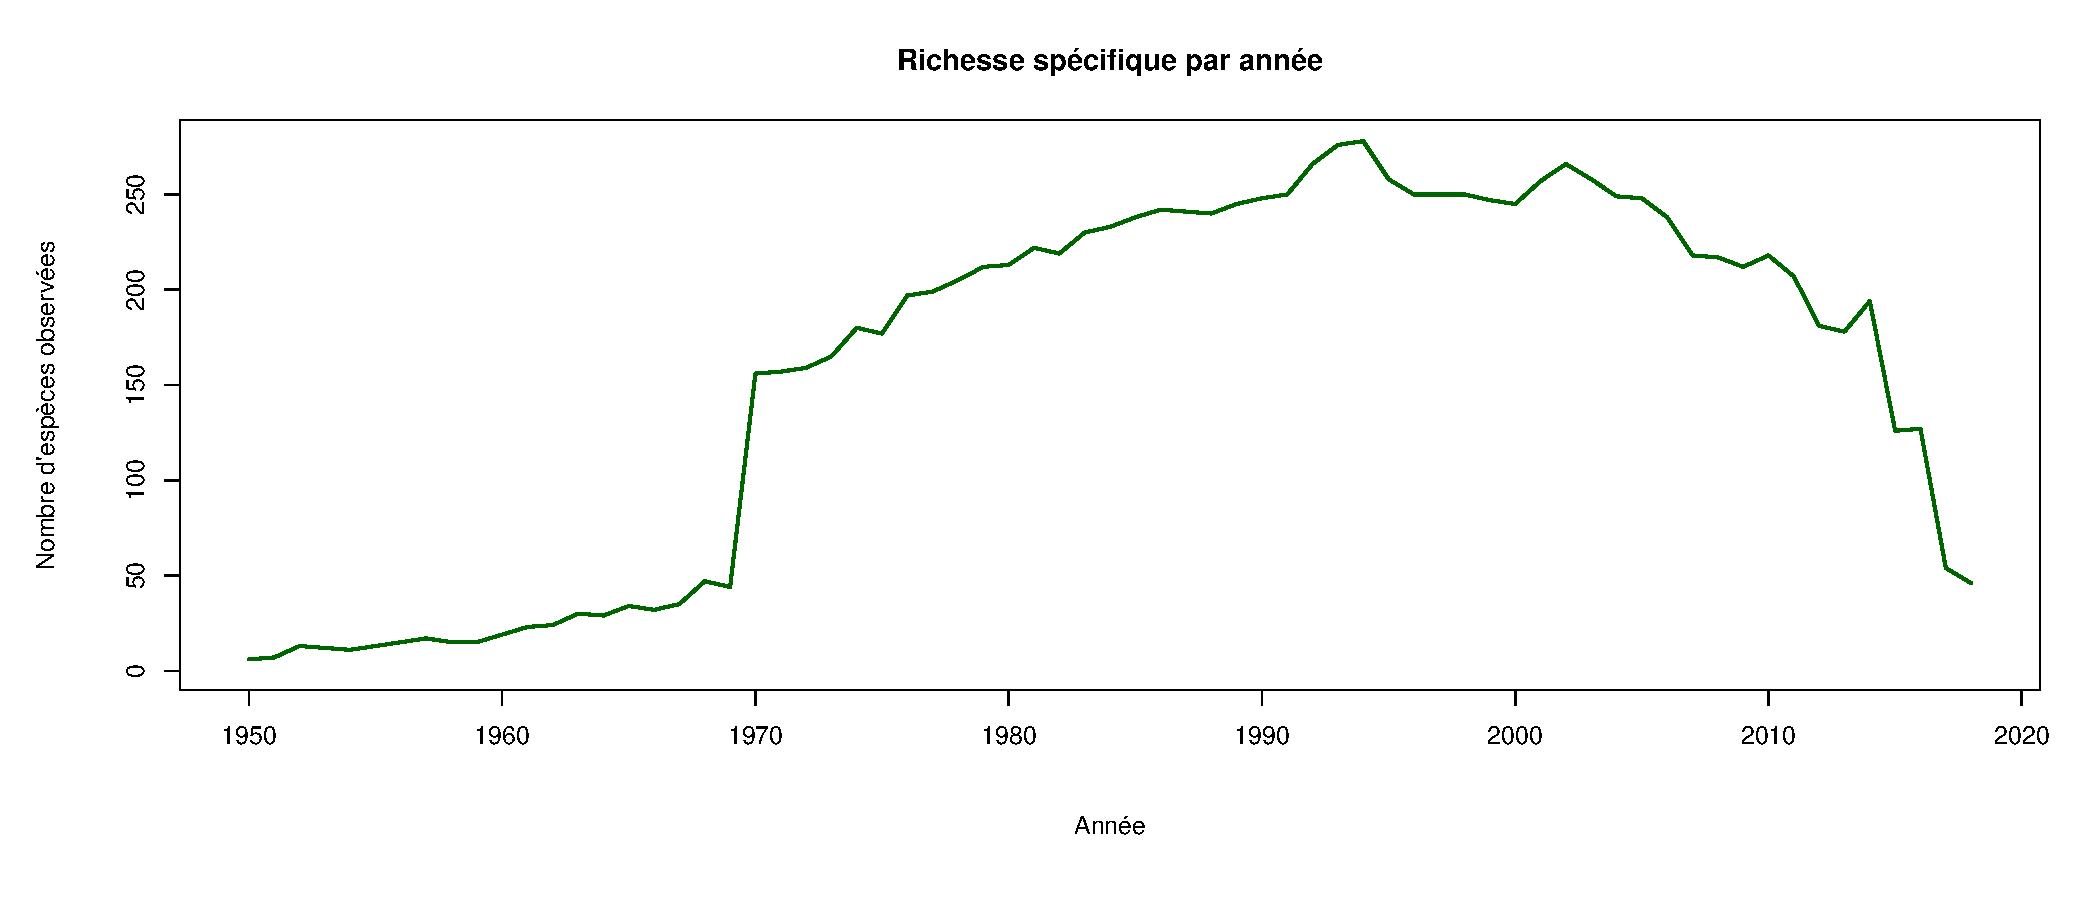
\includegraphics[width=1\linewidth]{../Figures/figure_1_esp_par_annee} \caption{\label{fig:esp.annee} Richesse spécifique par année}\label{fig:fig.esp.annee}
\end{figure}

La Figure \ref{fig:obs.classe} mets en évidence les observations par
classe taxonomique sur une échelle logarithmique. Teleostei représente
la classe qui cumule le plus grand nombre total d'observation, à
l'opposé de Petromyzonti.

\begin{figure}
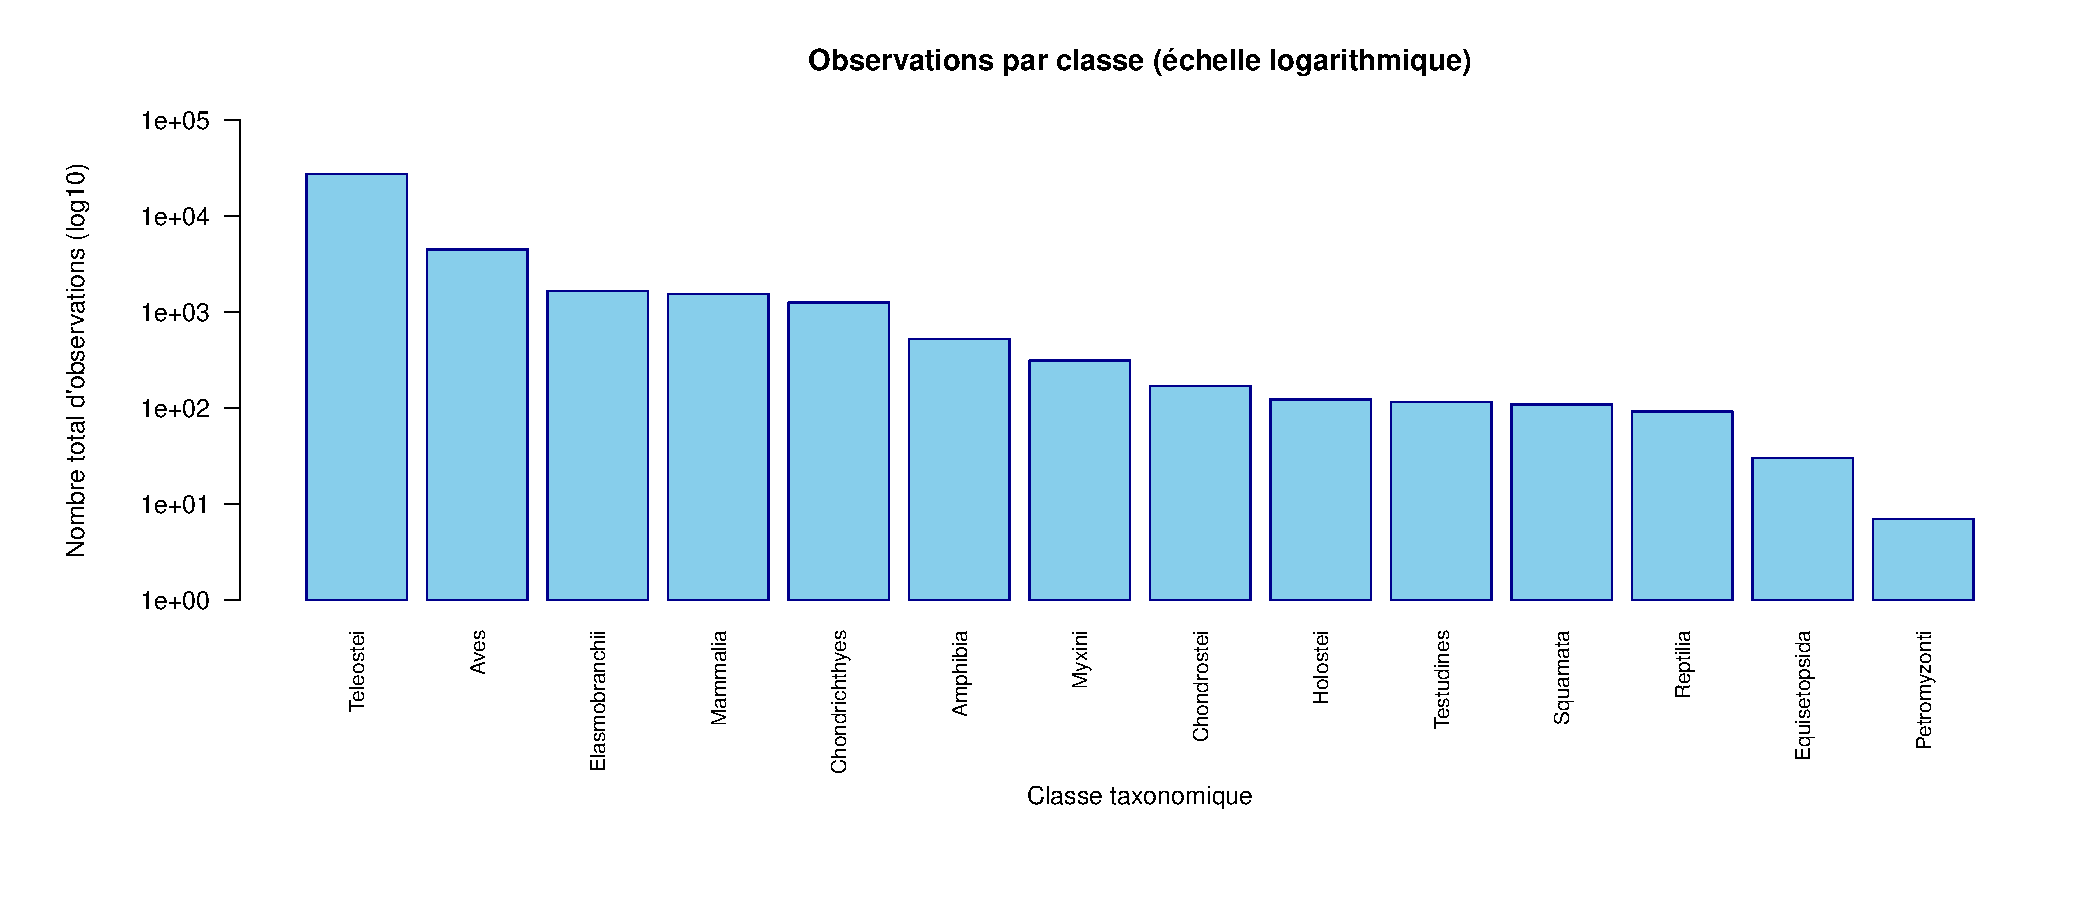
\includegraphics[width=1\linewidth]{../Figures/figure_2_obs_par_classe} \caption{\label{fig:obs.classe} Observations par classe (échelle logarithmique)}\label{fig:fig.obs.classe}
\end{figure}

Finalement, les variations en pourcentage des différentes classes
taxonomiques depuis les années 1970 sont montrées dans la Figure
\ref{fig:declin}. Les bandes vertes sont des valeurs positives
démontrant une augmentation d'espèces de cette classe et les bandes
rouges sont des diminutions dans le nombre d'espèces observées, donc des
valeurs négatives. Pour cette figure, la classe des Amphibia est celle
qui a la plus grande variation (500\%). Les classes Chondrostei et
Equisetopsida ont une valeur respective de 100\%. Dans les valeurs
négatives, la classe Aves est celle qui a la plus grande diminution avec
une valeur de - 99\%. Une valeur de 0 pour la classe des Petromyzonti
est également observée.

\begin{figure}
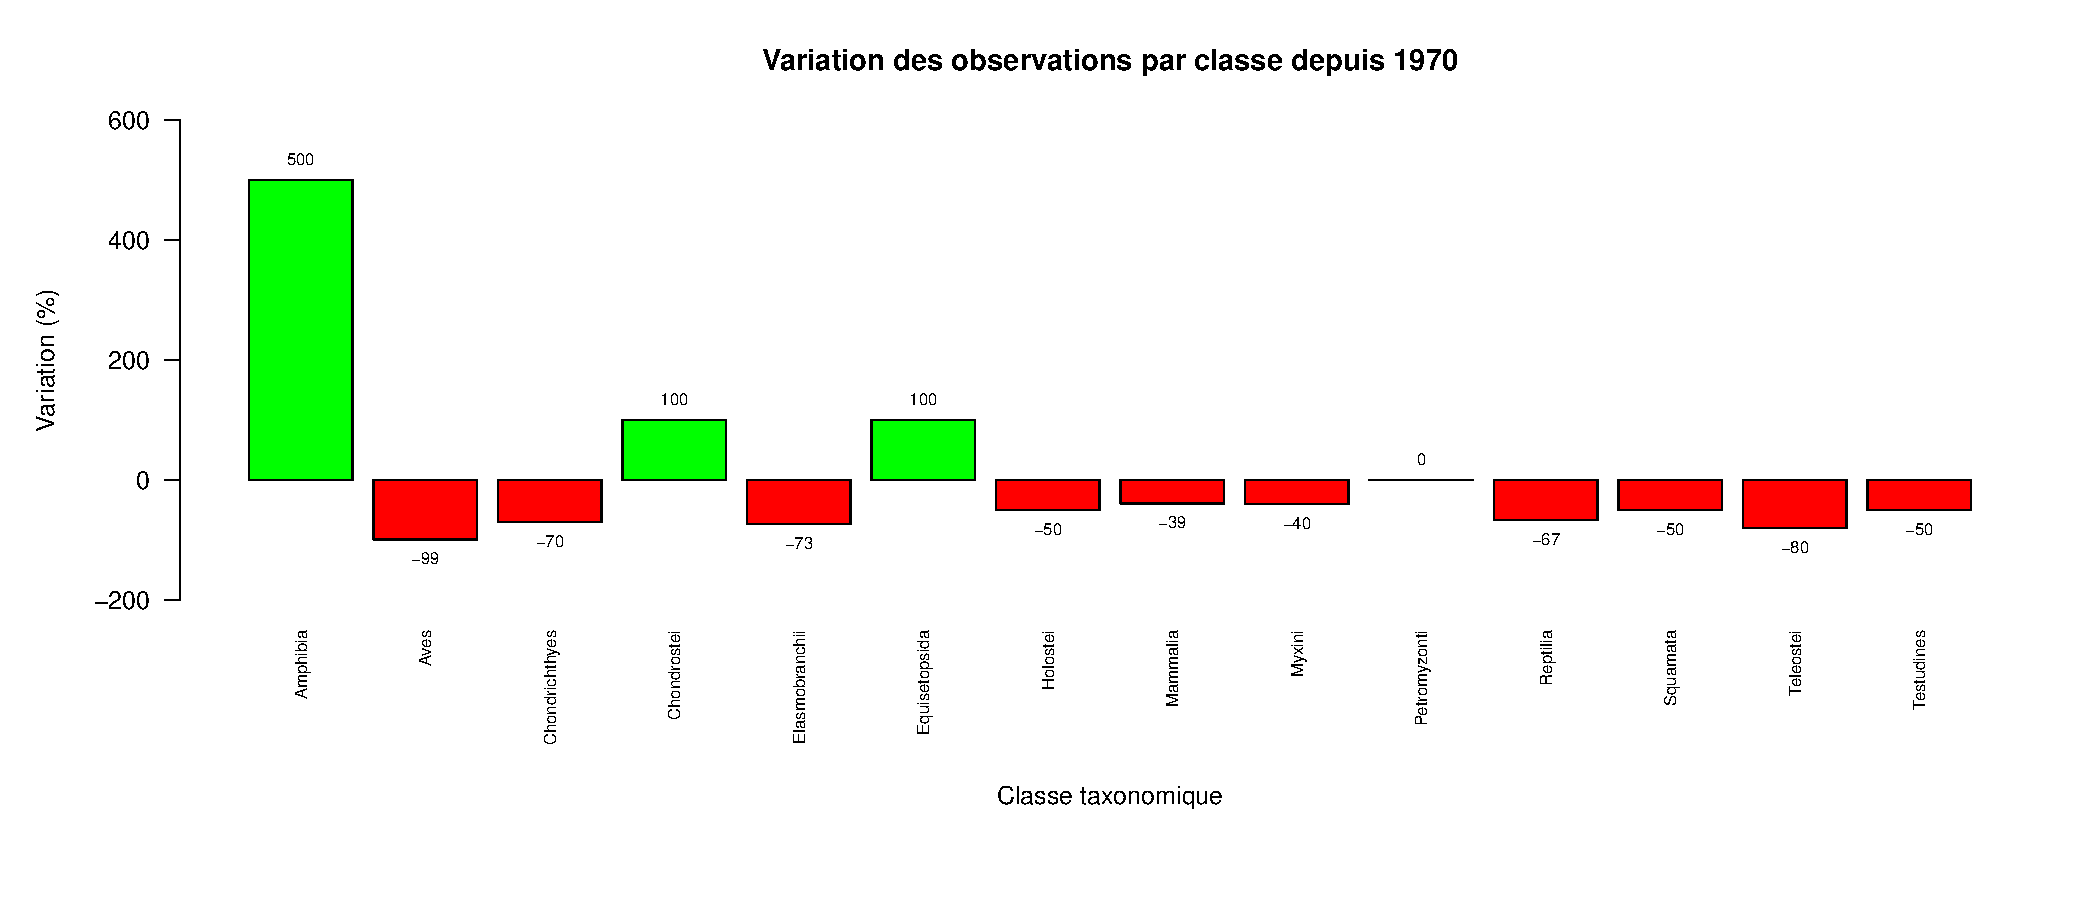
\includegraphics[width=1\linewidth]{../Figures/figure_3_declin_classe} \caption{\label{fig:declin} Variation des observations par classe depuis 1970}\label{fig:fig.declin}
\end{figure}

\section{Discussion}\label{discussion}

En ce qui concerne la première question de recherche, observe-t-on un
déclin de la biodiversité à travers les années, la Figure
\ref{fig:esp.annee} est la clé pour répondre. Entre les années 1950 et
1970 le nombre d'espèces observées est plus faible que les années
suivantes. Cette faible augmentation dans les observations, peut être
reliée à un manque d'échantillonnage ou simplement une abondance des
espèces étaient moins prononcée aux endroits étudiés. De plus, est
notable en 1970, une hausse dans le nombre d'observation de manière
drastique. Cette hausse se fait de façon constante jusqu'aux années
1993/1994. À partir de ces années, un déclin dans la richesse spécifique
est visible. Ce déclin pourrait être relié à l'endroit où les données
ont été récoltées car l'impact sur la biodiversité diffère selon les
biomes étudiés. Les biomes les plus sous représentés sont notamment les
forêts boréales, les toundras, les prairies inondées, les savanes ainsi
que les mangroves (2). Donc, les espèces retrouvées dans ces milieux
sont sujettes à un biais lié à l'emplacement de leur habitat. Depuis les
années 1980, des préoccupations sont levées à propos de la vitesse à
laquelle les espèces sont perdues de leurs écosystèmes (5). Le graphique
de la Figure \ref{fig:esp.annee}, met en évidence une diminution
constante dans le nombre d'observation à partir des années 2000. Donc,
un déclin dans la biodiversité à travers le temps est observé, causé par
l'activité humaine (4).

Pour répondre à la deuxième question de recherche qui consiste à
déterminer quel taxon a été le plus et le moins observé à travers les
années, la Figure \ref{fig:obs.classe} est utilisée. La classe Teleostei
cumule le plus grand nombre d'observations et Petromyzonti le moins
d'observations. Il est cependant important de considérer que lors des
analyses statistiques, l'unité d'échantillonnage utilisée n'était pas la
même pour chaque classe, ce qui peut avoir créé un biais lors des
analyses finales.

Dans le but de répondre à la dernière question de recherche, étant quel
taxon a le plus décliné depuis les années 1970, la Figure
\ref{fig:declin} est essentielle car elle permet d'observer les
différentes variations des observations selon la classe. Ainsi, c'est la
classe Aves, plus généralement considérée comme les oiseaux, qui a le
plus décliné avec une diminution de 99\%. Toutefois, les données pour
créer ce graphique incluent seulement les observations depuis les années
1970, puisqu'entre 1950 et 1970 il y avait très peu d'échantillons
récoltés. Alors, en considérant les données depuis 1970 un biais dans
l'analyse est créé. Comme démontré dans la littérature, les activités
anthropiques ne font qu'accélérer le déclin dans l'abondance des espèces
(4). Ce déclin est de plus en plus observé depuis les années 2010 où la
biodiversité, à l'échelle terrestre, diminue grandement et rapidement
(5).

\section{Conclusion}\label{conclusion}

Pour conclure, à travers le temps, une diminution dans la richesse
spécifique des différentes espèces retrouvées dans l'écosystème
terrestre est observée. Selon leur environnement, certaines espèces sont
plus susceptibles que d'autres à un déclin dans leur population. Malgré,
la reconnaissance des effets anthropiques sur les écosystèmes et leurs
espèces, l'Homme doit fortement augmenter ses efforts de conservation
afin d'assurer la conservation et la préservation des biomes.

\section*{Bibliographie}\label{bibliographie}
\addcontentsline{toc}{section}{Bibliographie}

\pnasbreak

\phantomsection\label{refs}
\begin{CSLReferences}{0}{1}
\bibitem[\citeproctext]{ref-kissling_building_2018}
\CSLLeftMargin{1. }%
\CSLRightInline{Kissling WD, et al. (2018)
\href{https://doi.org/10.1111/brv.12359}{Building essential biodiversity
variables of species distribution and abundance at a global scale}.
\emph{Biological Reviews} 93(1):600--625.}

\bibitem[\citeproctext]{ref-newbold_has_2016}
\CSLLeftMargin{2. }%
\CSLRightInline{Newbold T, et al. (2016)
\href{https://doi.org/10.1126/science.aaf2201}{Has land use pushed
terrestrial biodiversity beyond the planetary boundary? {A} global
assessment}. \emph{Science} 353(6296):288--291.}

\bibitem[\citeproctext]{ref-tittensor_mid-term_2014}
\CSLLeftMargin{3. }%
\CSLRightInline{Tittensor DP, et al. (2014)
\href{https://doi.org/10.1126/science.1257484}{A mid-term analysis of
progress toward international biodiversity targets}. \emph{Science}
346(6206):241--244.}

\bibitem[\citeproctext]{ref-matthews_review_2015}
\CSLLeftMargin{4. }%
\CSLRightInline{Matthews TJ, Whittaker RJ (2015)
\href{https://doi.org/10.1111/1365-2664.12380}{{REVIEW}: {On} the
species abundance distribution in applied ecology and biodiversity
management}. \emph{Journal of Applied Ecology} 52(2):443--454.}

\bibitem[\citeproctext]{ref-cardinale_biodiversity_2012}
\CSLLeftMargin{5. }%
\CSLRightInline{Cardinale BJ, et al. (2012)
\href{https://doi.org/10.1038/nature11148}{Biodiversity loss and its
impact on humanity}. \emph{Nature} 486(7401):59--67.}

\end{CSLReferences}



% Bibliography
% \bibliography{pnas-sample}

\end{document}
